\subsection{Single Variable Linear Regression}
We will first run our program on a single variable function of the form $y=5x_1$ through the following code.
\begin{lstlisting}
    ##Single Variable
    #GENERATE SAMPLE DATA
    X = generate_in(100, 1)
    Coeff = Matrix([[5]])
    Y = generate_out(Coeff, X)
    
    # SOLVE FOR BETA USING NORMAL EQUATION
    BETA = (X.transpose() * X).inverse() * X.transpose() * Y
    
    #Plot Sample Data and Predicted Values
    one_variable(Y,X,BETA)
    
\end{lstlisting}
This will generate a data sample of size 1000 and 1 feature with additional noise giving us data in figure 1(a). Next we will compute the line of best fit using BETA and plot the data and the line of best fit as shown in figure 1(b).   

\begin{figure}[h!]
    \centering
    \begin{subfigure}{0.5\textwidth}
        \centering
        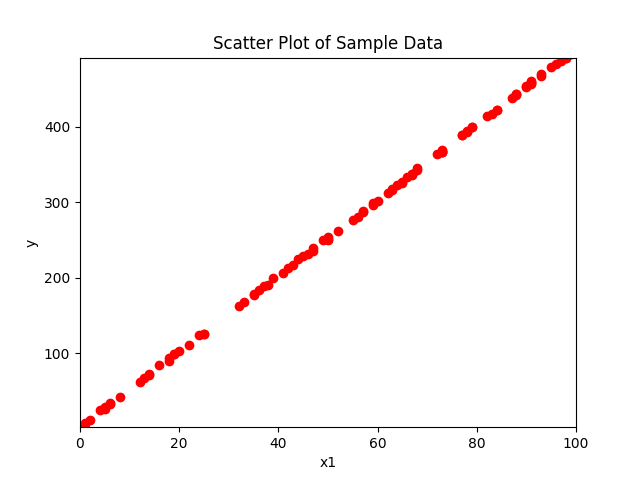
\includegraphics[scale=0.4]{One Variable Original.png}
        \caption{Original Data Set}
    \end{subfigure}%
    \begin{subfigure}{0.5\textwidth}
        \centering
        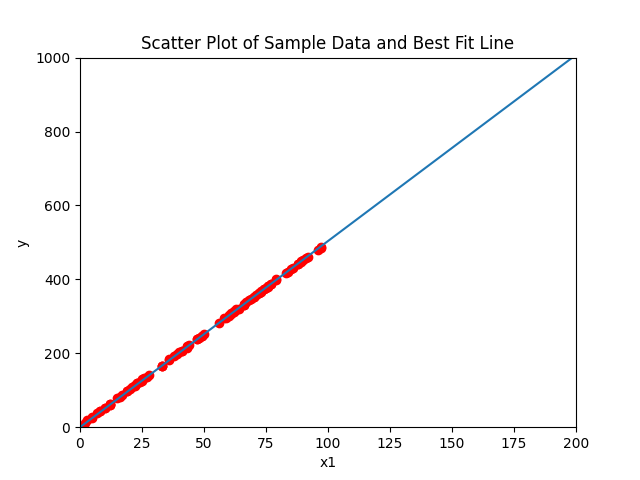
\includegraphics[scale=0.4]{One Variable Best Fit.png}
        \caption{Original Data Set and Line of Best Fit} 
    \end{subfigure}
    \caption{Single Variable Linear Regression}
\end{figure} 
\noindent The function \textit{one\_variable} which is responsible for plotting the data and the line of best fit is shown below.
\begin{lstlisting}
    def one_variable(Y,X,beta):
        x1 = [0] *(X.m)
        y=[0] *(Y.m)
        for i in range (X.m):
            x1[i]=X.matrix[i][0]
        for i in range (Y.m):
            y[i]=Y.matrix[i][0]
        ynew=[beta.matrix[0][0]*x1 for x1 in range(200)]
        plt.plot(x1,y,'ro')
        plt.plot([i for i in range(200)],ynew)
        plt.title('Scatter Plot of Sample Data and Best Fit Line')
        plt.xlabel('x1')
        plt.ylabel('y')
        plt.axis((0,200,0,1000))
        plt.show()
\end{lstlisting}


\subsection{Multi-Variable Linear Regression}
Next we will run our program for a multivariable function. Firstly we will generate data of sample size 1000 and 2 features.
We will use an equation of the form $y=5x_1+3x_2$ and generate sample outputs using the inputs and the coeffecients and use the normal equation to solve for BETA.
\begin{lstlisting}
    ##Multivariable
    #GENERATE SAMPLE DATA
    X=generate_in(1000,2)
    Coeff=Matrix([[5],[3]])
    Y=generate_out(Coeff,X)
    #SOLVE FOR BETA USING NORMAL EQUATION
    BETA=(X.transpose()*X).inverse()*X.transpose()*Y
    
    ##GRAPH CONTOUR PLOT
    mesh_grid(BETA)
    two_variable(X,Y)
\end{lstlisting}
We will use a contour plot to visualize the data and the approximation of the function. Figure 2(a) shows the original data set and figure 2(b) shows predicted values generated by linear regression.
\begin{figure}[H]
    \centering
    \begin{subfigure}{0.5\textwidth}
        \centering
        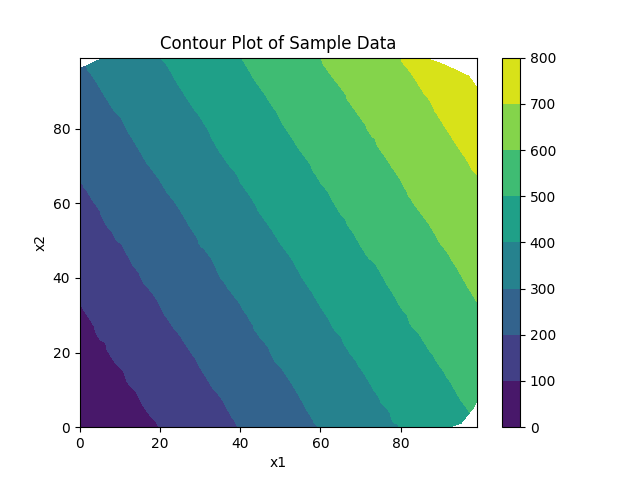
\includegraphics[scale=0.4]{Two Variable Original.png}
        \caption{Original Data Set}
    \end{subfigure}%
    \begin{subfigure}{0.5\textwidth}
        \centering
        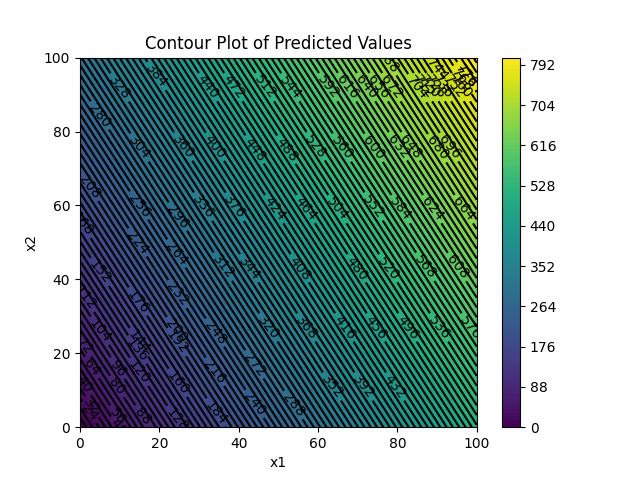
\includegraphics[scale=0.4]{Two Variable Predicted.png}
        \caption{Original Data Set and Predicted Values} 
    \end{subfigure}
    \caption{Multiple Variable Linear Regression}
\end{figure} 

\noindent The function \textit{two\_variable} will be used to plot the original sample data and the the function \textit{mesh\_grid} will be used to plot the contour plot of the predicted function both of which are shown below.
\begin{lstlisting}
    def mesh_grid(beta):
        x1=np.arange(0,101,1)
        x2=np.arange(0,101,1)
        X1,X2=np.meshgrid(x1,x2)
        Y=beta.matrix[0]*X1+beta.matrix[1]*X2
        ctr = plt.contour(X1, X2, Y, levels=100, colors='k')
        fil = plt.contourf(X1, X2, Y, levels=100)
        plt.clabel(ctr)
        plt.colorbar(fil)
        plt.show()

    def two_variable(X,Y):
        x1=[0]*X.m
        x2=[0]*X.m
        y = [0] * Y.m
        for i in range (X.m):
            x1[i]=X.matrix[i][0]
            x2[i]=X.matrix[i][1]
        for i in range (Y.m):
            y[i]=Y.matrix[i][0]
        plt.tricontourf(x1, x2, y)
        plt.colorbar()
        plt.show()
\end{lstlisting}